%%%%%%%%%%%%%%%%%%%%%%%%%%%%%%%%%%%%%%%%%%%%%%%%%%%%%%%%%%%%
%%  This Beamer template was created by Cameron Bracken.
%%  Anyone can freely use or modify it for any purpose
%%  without attribution.
%%
%%  Last Modified: January 9, 2009
%%

\documentclass[xcolor=x11names,compress]{beamer}

%% General document %%%%%%%%%%%%%%%%%%%%%%%%%%%%%%%%%%
\usepackage{graphicx}

\usepackage{xcolor}

\usepackage{pgffor} 

\usepackage{multimedia}

%%%%%%%%%%%%%%%%%%%%%%%%%%%%%%%%%%%%%%%%%%%%%%%%%%%%%%

\usepackage[frenchb]{babel}

\usepackage[utf8]{inputenc}

\usepackage{lastpage}

\usepackage[natbib=true, bibstyle=authoryear,
citestyle=authoryear, backend=bibtex]{biblatex}

\usepackage{caption}
\captionsetup{figurename=}

\usepackage{appendixnumberbeamer}

\resetcounteronoverlays{lstnumber}

%% Beamer Layout %%%%%%%%%%%%%%%%%%%%%%%%%%%%%%%%%%
\useoutertheme[subsection=false,shadow]{miniframes}
\useinnertheme{default} \usefonttheme{serif} 
\usepackage{palatino}

\setbeamerfont{title like}{shape=\scshape}
\setbeamerfont{title}{shape=\scshape}
\setbeamerfont{frametitle}{shape=\scshape}
\setbeamerfont{footline}{shape=\scshape}

\definecolor{MRed}{HTML}{8B0000} \definecolor{MGreen}{HTML}{008B00}
\definecolor{MBlue}{HTML}{00688B}

\setbeamercolor*{lower separation line head}{bg=MBlue}
\setbeamercolor*{normal text}{fg=black,bg=white}
\setbeamercolor*{alerted text}{fg=red} \setbeamercolor*{example
  text}{fg=black} \setbeamercolor*{structure}{fg=black}

\setbeamercolor*{palette tertiary}{fg=black,bg=black!10}
\setbeamercolor*{palette quaternary}{fg=black,bg=black!10}

\setbeamercolor{footlinerule}{bg=MBlue}
\setbeamercolor*{footlinecolor}{bg=black!10}

\setbeamercolor{block title}{use=structure,fg=white,bg=MBlue!75!black}
\setbeamercolor{block body}{use=structure,fg=black,bg=MBlue!20!white}

\setbeamercolor{block title
  example}{use=structure,fg=white,bg=MGreen!75!black}
\setbeamercolor{block body
  example}{use=structure,fg=black,bg=MGreen!20!white}

\setbeamercolor{block title
  alerted}{use=structure,fg=white,bg=MRed!75!black}
\setbeamercolor{block body
  alerted}{use=structure,fg=black,bg=MRed!20!white}

\renewcommand{\(}{\begin{columns}} \renewcommand{\)}{\end{columns}}
\newcommand{\<}[1]{\begin{column}{#1}} \renewcommand{\>}{\end{column}}
%%%%%%%%%%%%%%%%%%%%%%%%%%%%%%%%%%%%%%%%%%%%%%%%%%


\author{Arnaud Bletterer} \title{Outils multidimensionnels de
  déformation}

\newcommand{\mytext}{Outils multidimensionnels de déformation}

\graphicspath{{PresentationFigs/}}

%%%%%%%%%%%%%%%%%%%%%%%%%%%%%%%%%%%%%%%%%%%%%%%%%%%%%%
%%%%%%%%%%%%%%%%%%%%%%%%%%%%%%%%%%%%%%%%%%%%%%%%%%%%%%

\makeatother \setbeamertemplate{footline} {%
  \leavevmode
  \begin{beamercolorbox}[wd=\paperwidth,ht=1ex,dp=0ex,center]{footlinerule}
  \end{beamercolorbox}%



  \hbox{\begin{beamercolorbox}[wd=1\paperwidth,ht=2.5ex,dp=1.125ex,leftskip=.3cm,rightskip=.3cm]{footlinecolor}%
      \count1 = \linewidth \divide\count1 by \inserttotalframenumber

      \foreach \n in {1,...,\insertframenumber}{\hskip1.\count1}
      
\includegraphics[scale=0.06, viewport= 400 200 0 0]{cgogn}
   
  \end{beamercolorbox}
}

\hbox{\begin{beamercolorbox}[wd=.5\paperwidth,ht=2.5ex,dp=1.125ex,leftskip=.3cm,rightskip=.3cm]{footlinecolor}%
    \inserttitle
  \end{beamercolorbox}%

    \begin{beamercolorbox}[wd=.5\paperwidth,ht=2.5ex,dp=1.125ex,leftskip=.3cm,rightskip=.3cm]{footlinecolor}%
      \usebeamerfont{author in head/foot}\insertauthor\hfill
      \insertframenumber /\inserttotalframenumber
    \end{beamercolorbox}}%
  \vskip0pt%
} \makeatletter

%%%%%%%%%%%%%%%%%%%%%%%%%%%%%%%%%%%%%%%%%%%%%%%%%%%%%%
%%%%%%%%%%%%%%%%%%%%%%%%%%%%%%%%%%%%%%%%%%%%%%%%%%%%%%

\newcommand{\highlightR}[1]{%
  \colorbox{MRed!50}{$\displaystyle#1$}} \newcommand{\highlightB}[1]{%
  \colorbox{MBlue!50}{$\displaystyle#1$}}
\newcommand{\highlightG}[1]{%
  \colorbox{MGreen!50}{$\displaystyle#1$}}
\newcommand{\highlightO}[1]{%
  \colorbox{orange!50}{$\displaystyle#1$}}
\newcommand{\highlightV}[1]{%
  \colorbox{violet!50}{$\displaystyle#1$}}
\newcommand{\highlightGR}[1]{%
  \colorbox{gray!50}{$\displaystyle#1$}}

\bibliography{../Rapport/References/references.bib}
\begin{document}

%%%%%%%%%%%%%%%%%%%%%%%%%%%%%%%%%%%%%%%%%%%%%%%%%%%%%%
%%%%%%%%%%%%%%%%%%%%%%%%%%%%%%%%%%%%%%%%%%%%%%%%%%%%%%
\begin{frame}
  \title{Outils multidimensionnels de déformation\\~\\

    \begin{figure}
      \begin{center}
        
\includegraphics[scale=0.3]{uds-logo}~~~~~~~~~
        
\includegraphics[scale=0.15]{icube-logo}
      \end{center}
    \end{figure}
  } \author{Arnaud Bletterer \\ \textit{Université de Strasbourg}
    \vspace{-0.5cm} \date{\today} } \titlepage
\end{frame}

%%%%%%%%%%%%%%%%%%%%%%%%%%%%%%%%%%%%%%%%%%%%%%%%%%%%%%
%                    INTRODUCTION                    %
%%%%%%%%%%%%%%%%%%%%%%%%%%%%%%%%%%%%%%%%%%%%%%%%%%%%%%

\section{\scshape Introduction}

\begin{frame}{Déformation spatiale}
  \begin{columns}[t]
    \begin{column}{0.5\textwidth}
      \centering
      
\includegraphics[scale=0.16]{Outil-Mono-Sans}
    \end{column}
    \begin{column}{0.5\textwidth}
      \centering
      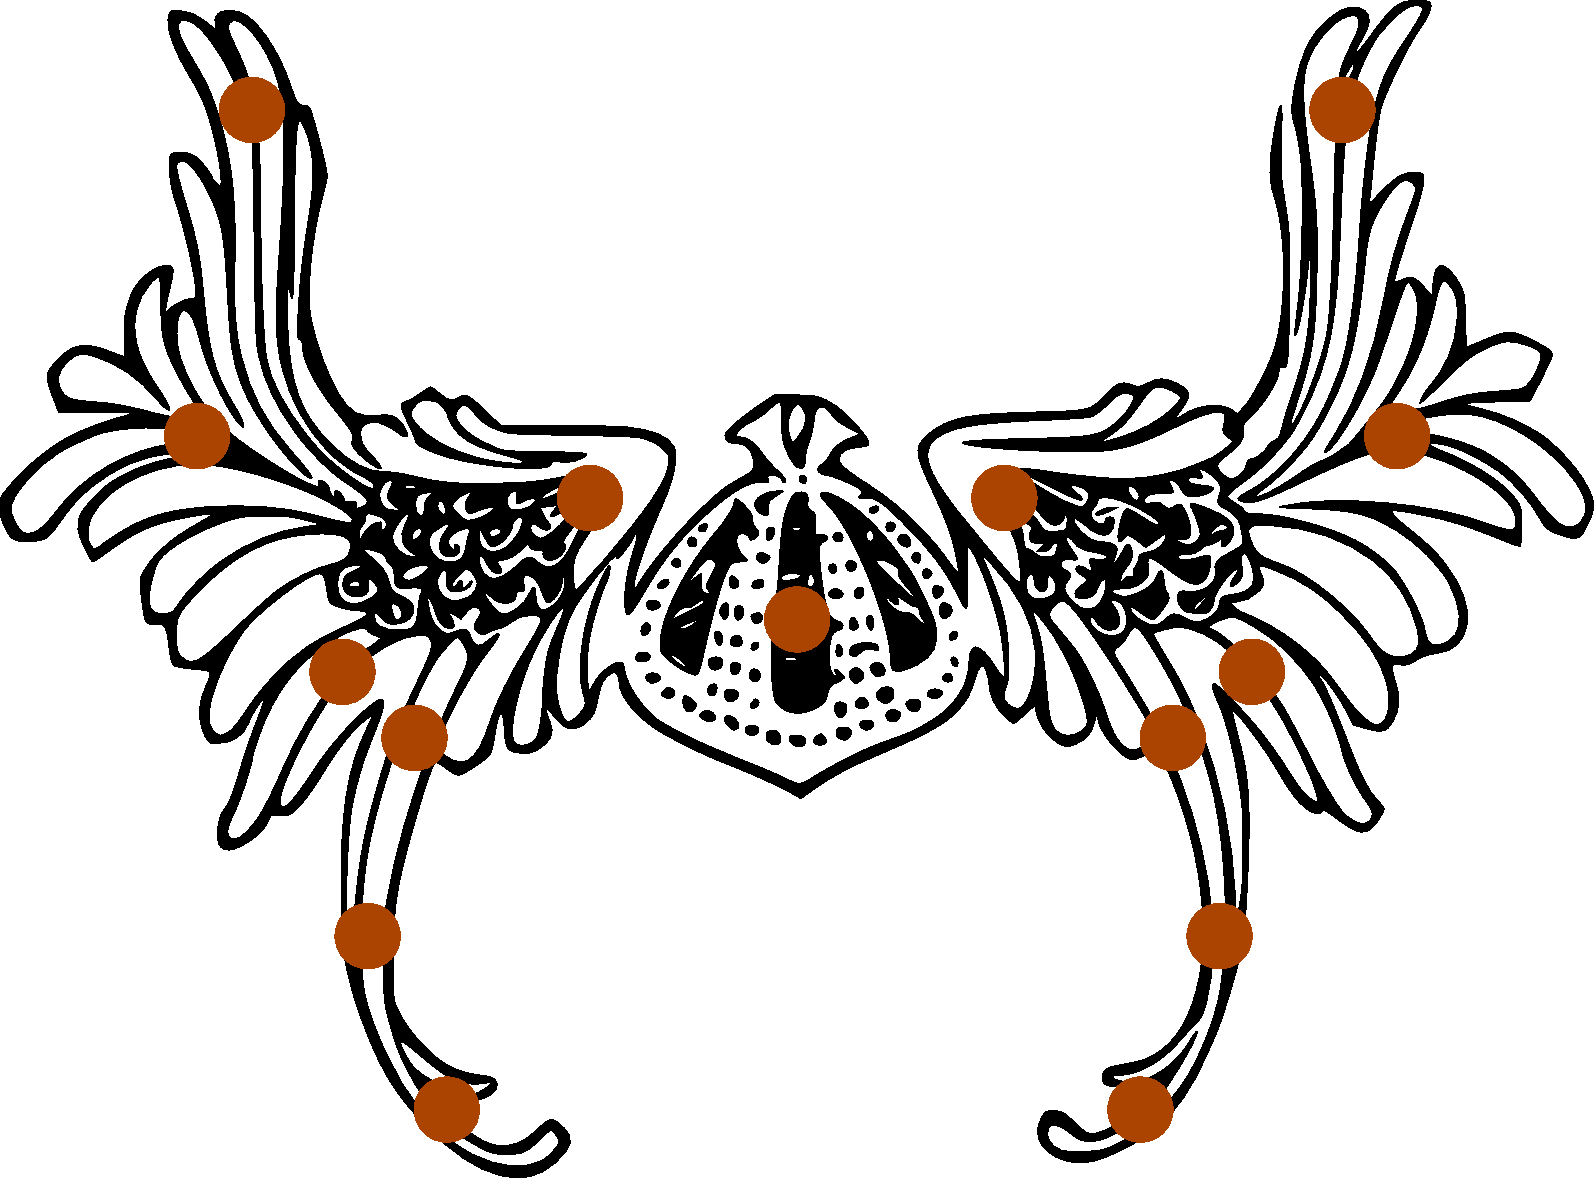
\includegraphics[scale=0.16]{Outil-Mono-Points}
    \end{column}
  \end{columns}
  \begin{block}{Etapes}
    \begin{enumerate}
      \item Création de l'outil
      \item Association des points de l'espace à l'outil
      \item Déformation de l'objet par invariance de l'association
    \end{enumerate}
  \end{block}
\end{frame}

\begin{frame}{Outils de déformation}
  \begin{exampleblock}{Propriétés}
    \setbeamercolor{itemize item}{fg=MGreen}
    \begin{itemize}
      \item Dimension : Point, Courbe, Surface, Volume
      \item Résolution : Nombre de points de contrôle
      \item Influence : Locale ou Globale
    \end{itemize}
  \end{exampleblock}
  \centering
  \begin{columns}[t]
    \begin{column}{0.3\textwidth}
    \centering
      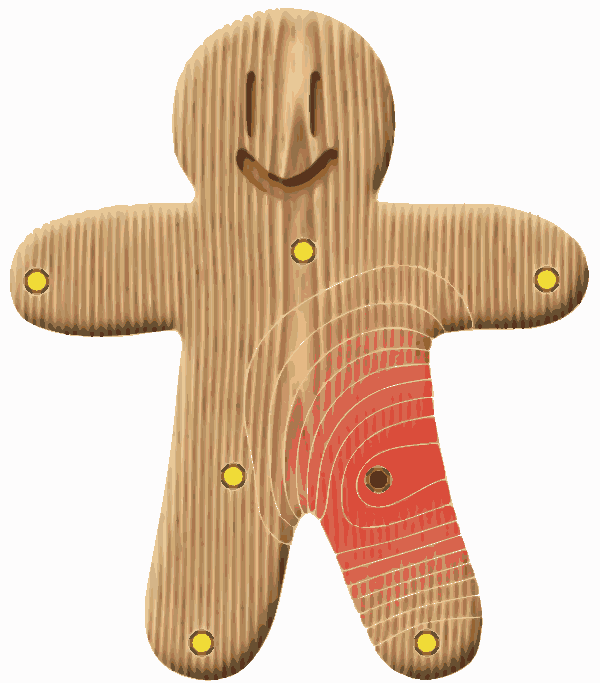
\includegraphics[scale=0.25]{Bounded-InfluenceLocale}
    \end{column}
    \begin{column}{0.3\textwidth}
    \centering
      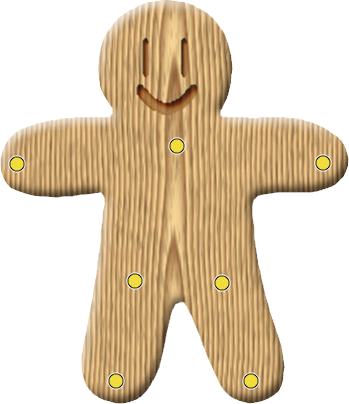
\includegraphics[scale=0.25]{Bounded-InfluenceGlobale}
    \end{column}
  \end{columns}
\end{frame}

\begin{frame}{Objectifs multi-outil}
  \centering  
  \includegraphics[scale=0.3]<1>{Outil-Mono-Sans}
  \includegraphics[scale=0.3]<2>{Outil-Courbe}
  \includegraphics[scale=0.3]<3>{Outil-CourbeSurface}
  \includegraphics[scale=0.3]<4>{Outil-PointCourbeSurface}
\end{frame}

\begin{frame}{Bounded Biharmonic Weights for Real-Time Deformation 
$_{[\text{\cite{JBPS11}}]}$}

  \begin{itemize}
    \item Mélange d'outils de différentes dimensions
    \item Méthode d'optimisation globale
  \end{itemize}
  \centering
  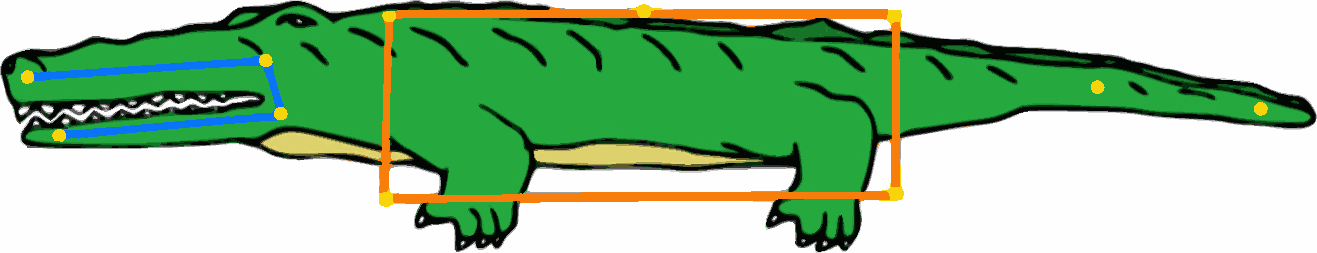
\includegraphics[scale=0.25]{Alligator-avant}
  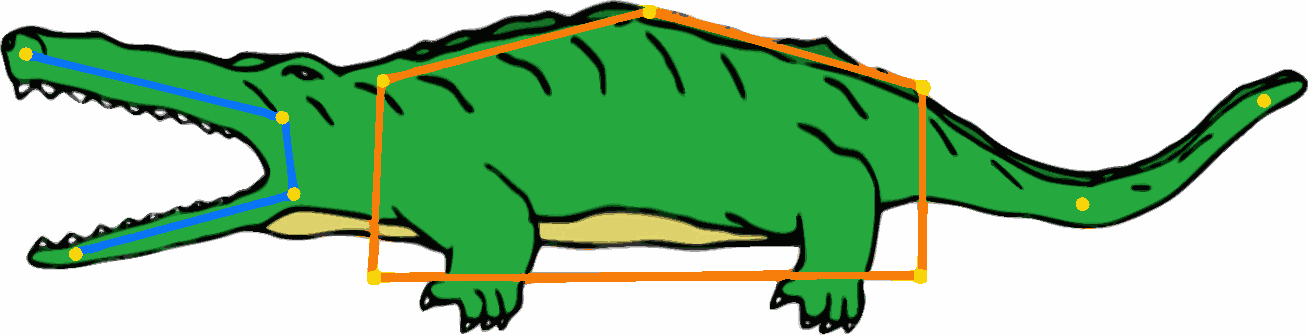
\includegraphics[scale=0.25]{Alligator-apres}
  \begin{alertblock}{Points négatifs}
  \setbeamercolor{itemize item}{fg=MRed}  
    \begin{itemize}
    \item Long temps d'association (discrétisation de l'espace)
    \item Modification d'un outil $\Rightarrow$ Recommencer l'association
    \end{itemize}
  \end{alertblock}
\end{frame}

\begin{frame}{*Cages : A Multilevel, Multi-cage based System for Mesh Deformation 
  $_{[\text{\cite{GPCP13}}]}$}
  \begin{columns}[T]
    \begin{column}{0.5\textwidth}
      \begin{itemize}
        \item Mélange d'outils existants
        \item Pavage de l'espace
        \item Chaque cage modifie une partie de l'objet
      \end{itemize}
      \begin{alertblock}{Points négatifs}
        \setbeamercolor{itemize item}{fg=MRed}  
        \begin{itemize}
          \item Long temps d'association
          \item 1 seule dimension d'outil
          \item Couverture de tout l'objet
        \end{itemize}
      \end{alertblock}
    \end{column}
    \begin{column}{0.4\textwidth}
      \centering
      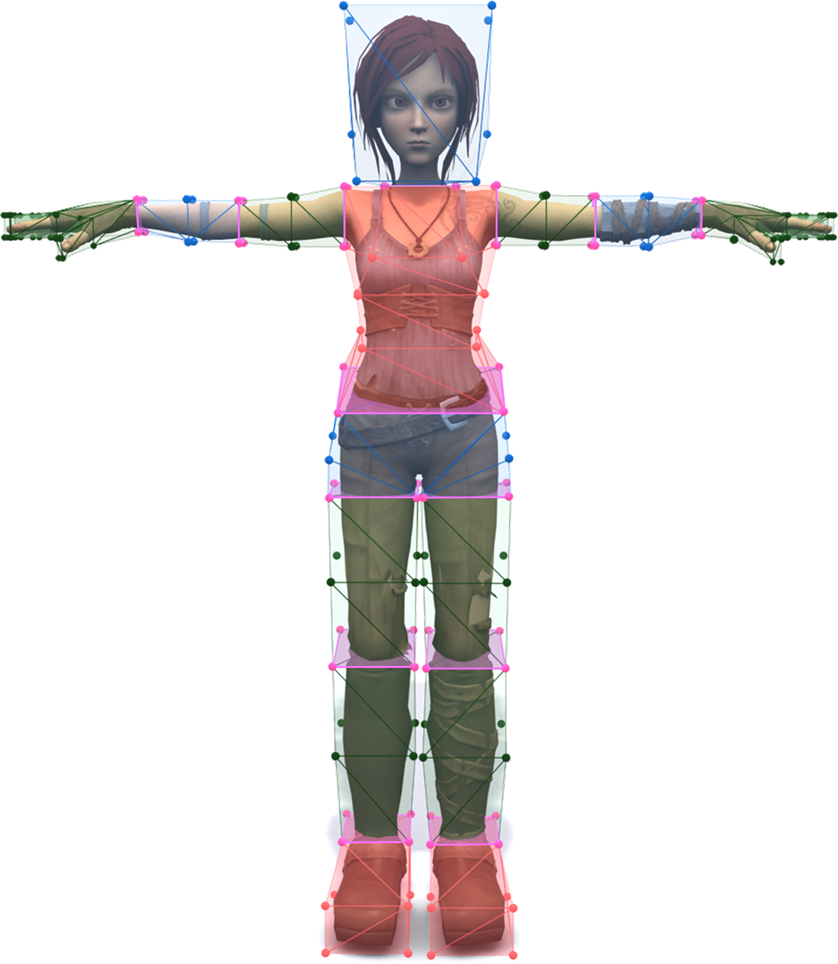
\includegraphics[scale=0.17]{starCages}
    \end{column}
  \end{columns}
\end{frame}

\begin{frame}{*Cages : A Multilevel, Multi-cage-based System for Mesh Deformation 
  $_{[\text{\cite{GPCP13}}]}$}
  \centering
  \begin{columns}[t]
    \begin{column}{0.3\textwidth}
      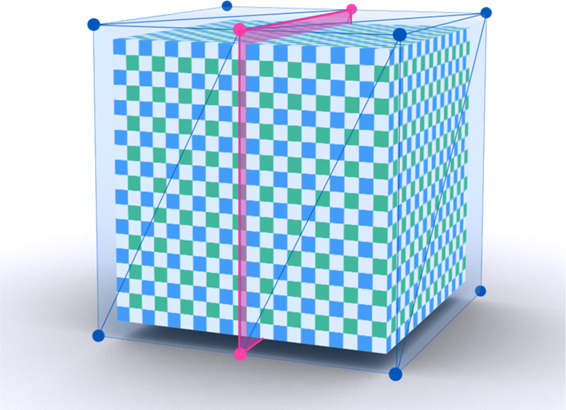
\includegraphics[scale=0.15]{starCages-Boite-Avant}
    \end{column}
    \begin{column}{0.3\textwidth}
      \centering
      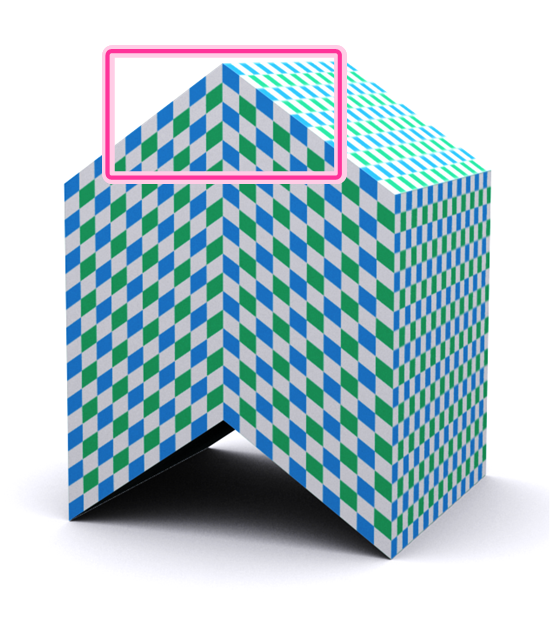
\includegraphics[scale=0.15]{starCages-Boite-Sans} \\
      \fcolorbox{magenta}{white}{
      \begin{minipage}{0.87\textwidth}
        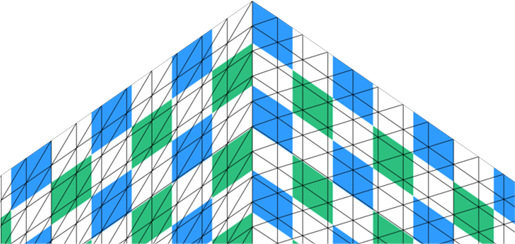
\includegraphics[scale=0.15]{starCages-Boite-Sans-Pres}
      \end{minipage}}
    \end{column}
    \begin{column}{0.3\textwidth}
      \centering
      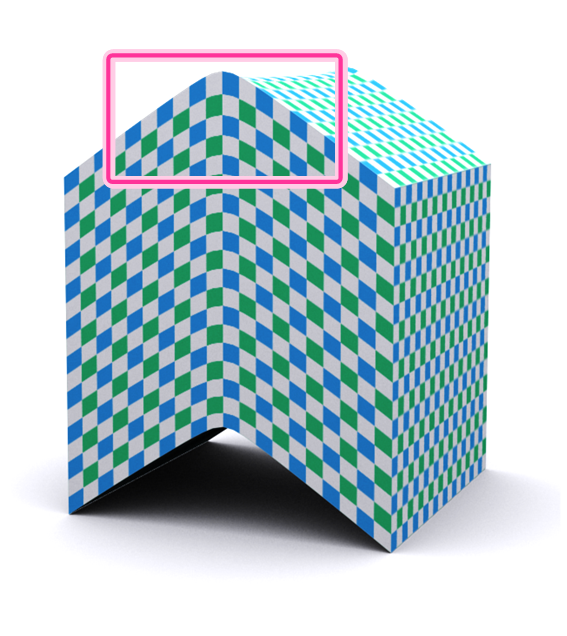
\includegraphics[scale=0.15]{starCages-Boite-Avec} \\
      \fcolorbox{magenta}{white}{
      \begin{minipage}{0.87\textwidth}
        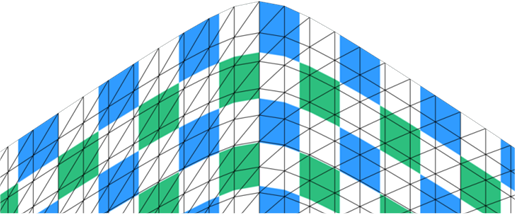
\includegraphics[scale=0.15]{starCages-Boite-Avec-Pres}
      \end{minipage}}
    \end{column}
  \end{columns}
\end{frame}

\begin{frame}{Objectifs}
\begin{itemize}
  \item Associer un outil à un sous-ensemble de points de l'espace
  \item Mélanger plusieurs outils sur un même objet
\end{itemize}
  \begin{block}{Fils directeurs}
    \begin{itemize}
      \item Minimisation des temps de calcul
      \item Formulations mathématiques simples et claires
    \end{itemize}
  \end{block}
\end{frame}

%%%%%%%%%%%%%%%%%%%%%%%%%%%%%%%%%%%%%%%%%%%%%%%%%%%%%%
%                  MELANGE D'OUTILS                  %
%%%%%%%%%%%%%%%%%%%%%%%%%%%%%%%%%%%%%%%%%%%%%%%%%%%%%%

\section{\scshape Contributions}

\begin{frame}{Déformation à base de cages}
\begin{columns}[T]
  \begin{column}{0.6\textwidth}
    \begin{displaymath}
      p = \sum_{i=1}^n \lambda_i v_i
    \end{displaymath}
    \begin{itemize}
      \item $[\lambda_1, ..., \lambda_n]$ sont les coordonnées barycentriques
      généralisées du point $p$
      \item Plusieurs méthodes pour obtenir ces coordonnées (MVC, HC, GC)
    \end{itemize}
  \end{column}
  \begin{column}{0.4\textwidth}
    \centering
    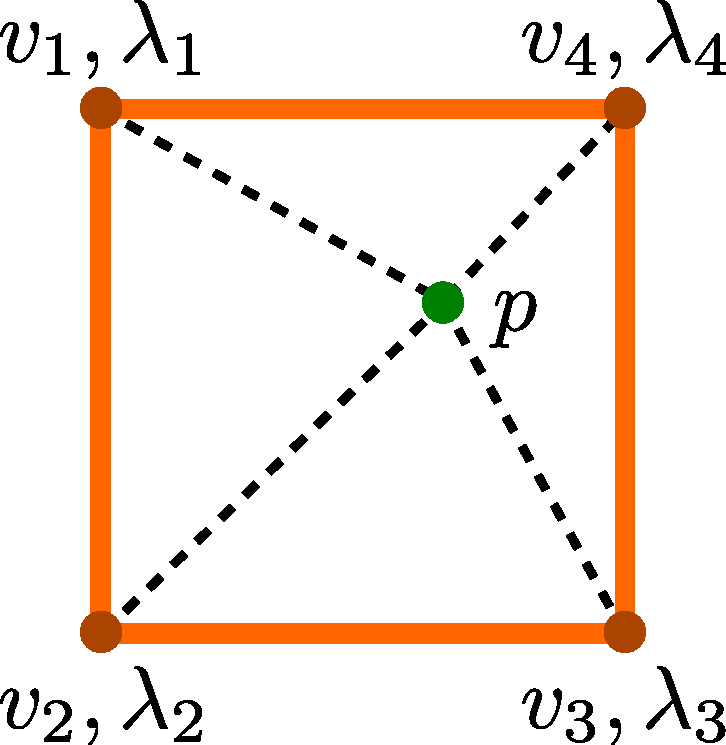
\includegraphics[scale=0.3]{Deformation-Cages}
  \end{column}
\end{columns}
\end{frame}

\begin{frame}{Problème actuel}
  \begin{columns}[t]
    \begin{column}{0.5\textwidth}
      \centering
      \includegraphics[scale=0.3]<1>{Deformation-Interieur-1Sommet-Avant}
      \includegraphics[scale=0.15]<2>{Deformation-Viking-Simple-Avant}
    \end{column}
    \begin{column}{0.5\textwidth}
      \centering
      \includegraphics[scale=0.3]<1>{Deformation-Interieur-1Sommet-Apres}
      \includegraphics[scale=0.15]<2>{Deformation-Viking-Simple-Sans}
    \end{column}
  \end{columns}
\end{frame}

\begin{frame}{Déformation partielle}
  \begin{itemize}
    \item Atténuer la déformation au bord de la cage
    \begin{displaymath}
      T_{d}(p) = \gamma(p) T(p) + (1-\gamma(p)) p
    \end{displaymath}
    \item Contrôle de l'atténuation
  \end{itemize}
  \begin{columns}[t]
    \begin{column}{0.3\textwidth}
      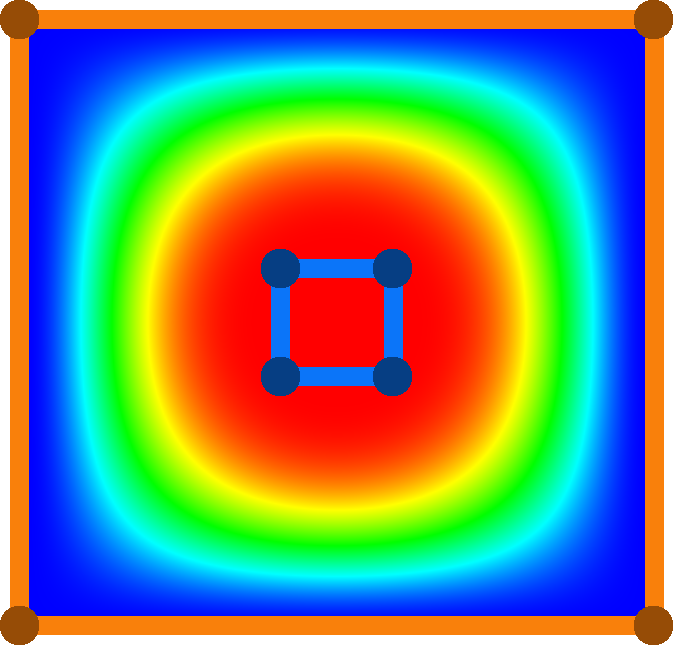
\includegraphics[scale=0.15]{BoundaryWeightFunction-Petite}
    \end{column}
    \begin{column}{0.3\textwidth}
      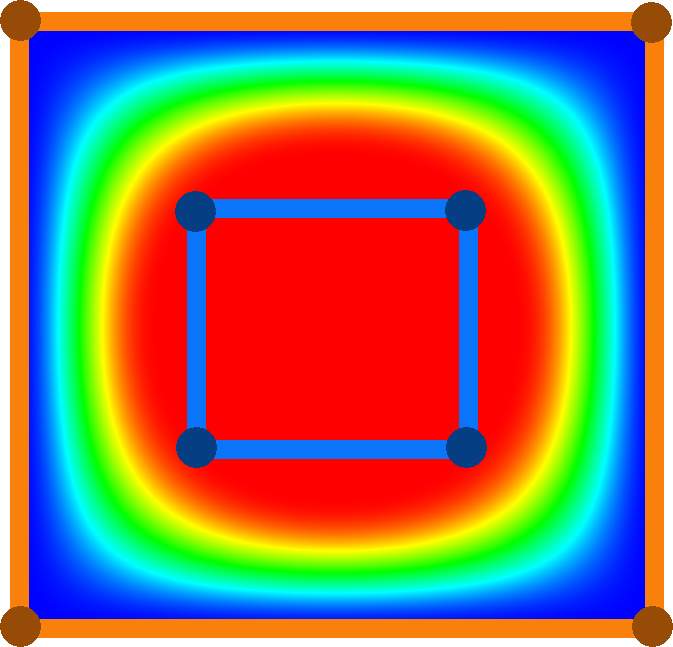
\includegraphics[scale=0.15]{BoundaryWeightFunction}
    \end{column}
    \begin{column}{0.3\textwidth}
      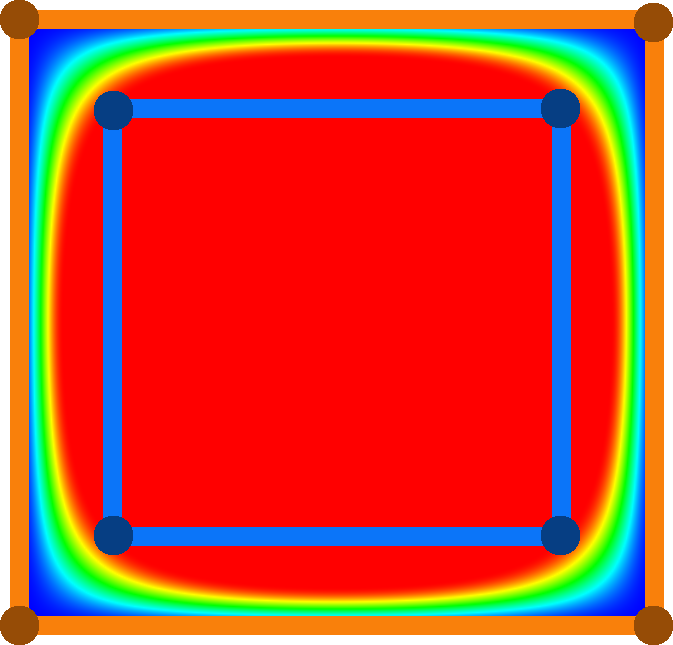
\includegraphics[scale=0.15]{BoundaryWeightFunction-Grande}
    \end{column}
  \end{columns}
\end{frame}

\begin{frame}{Résultat de l'atténuation}
  \begin{columns}[t]
    \begin{column}{0.5\textwidth}
      \centering
      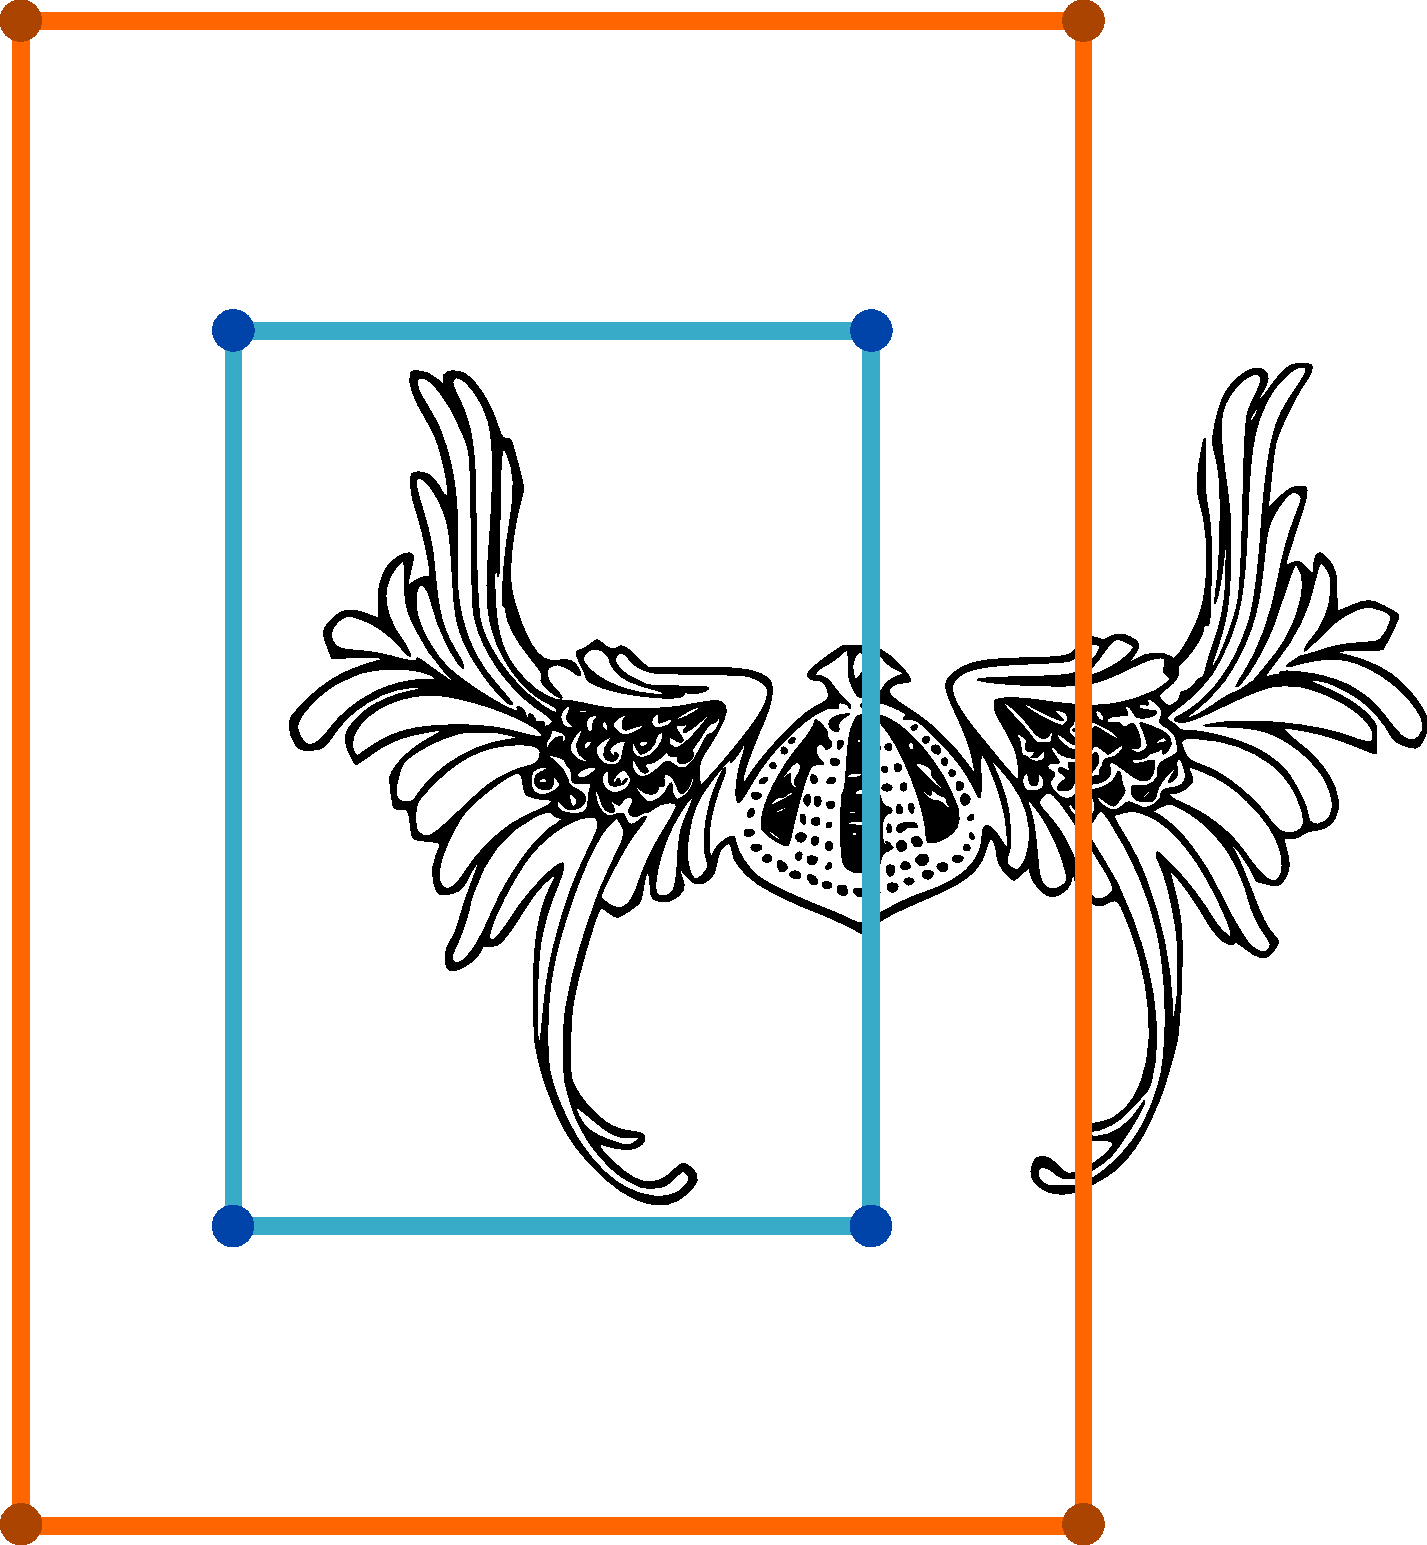
\includegraphics[scale=0.15]{Deformation-Viking-Double-Avant}
    \end{column}
    \begin{column}{0.5\textwidth}
      \centering
      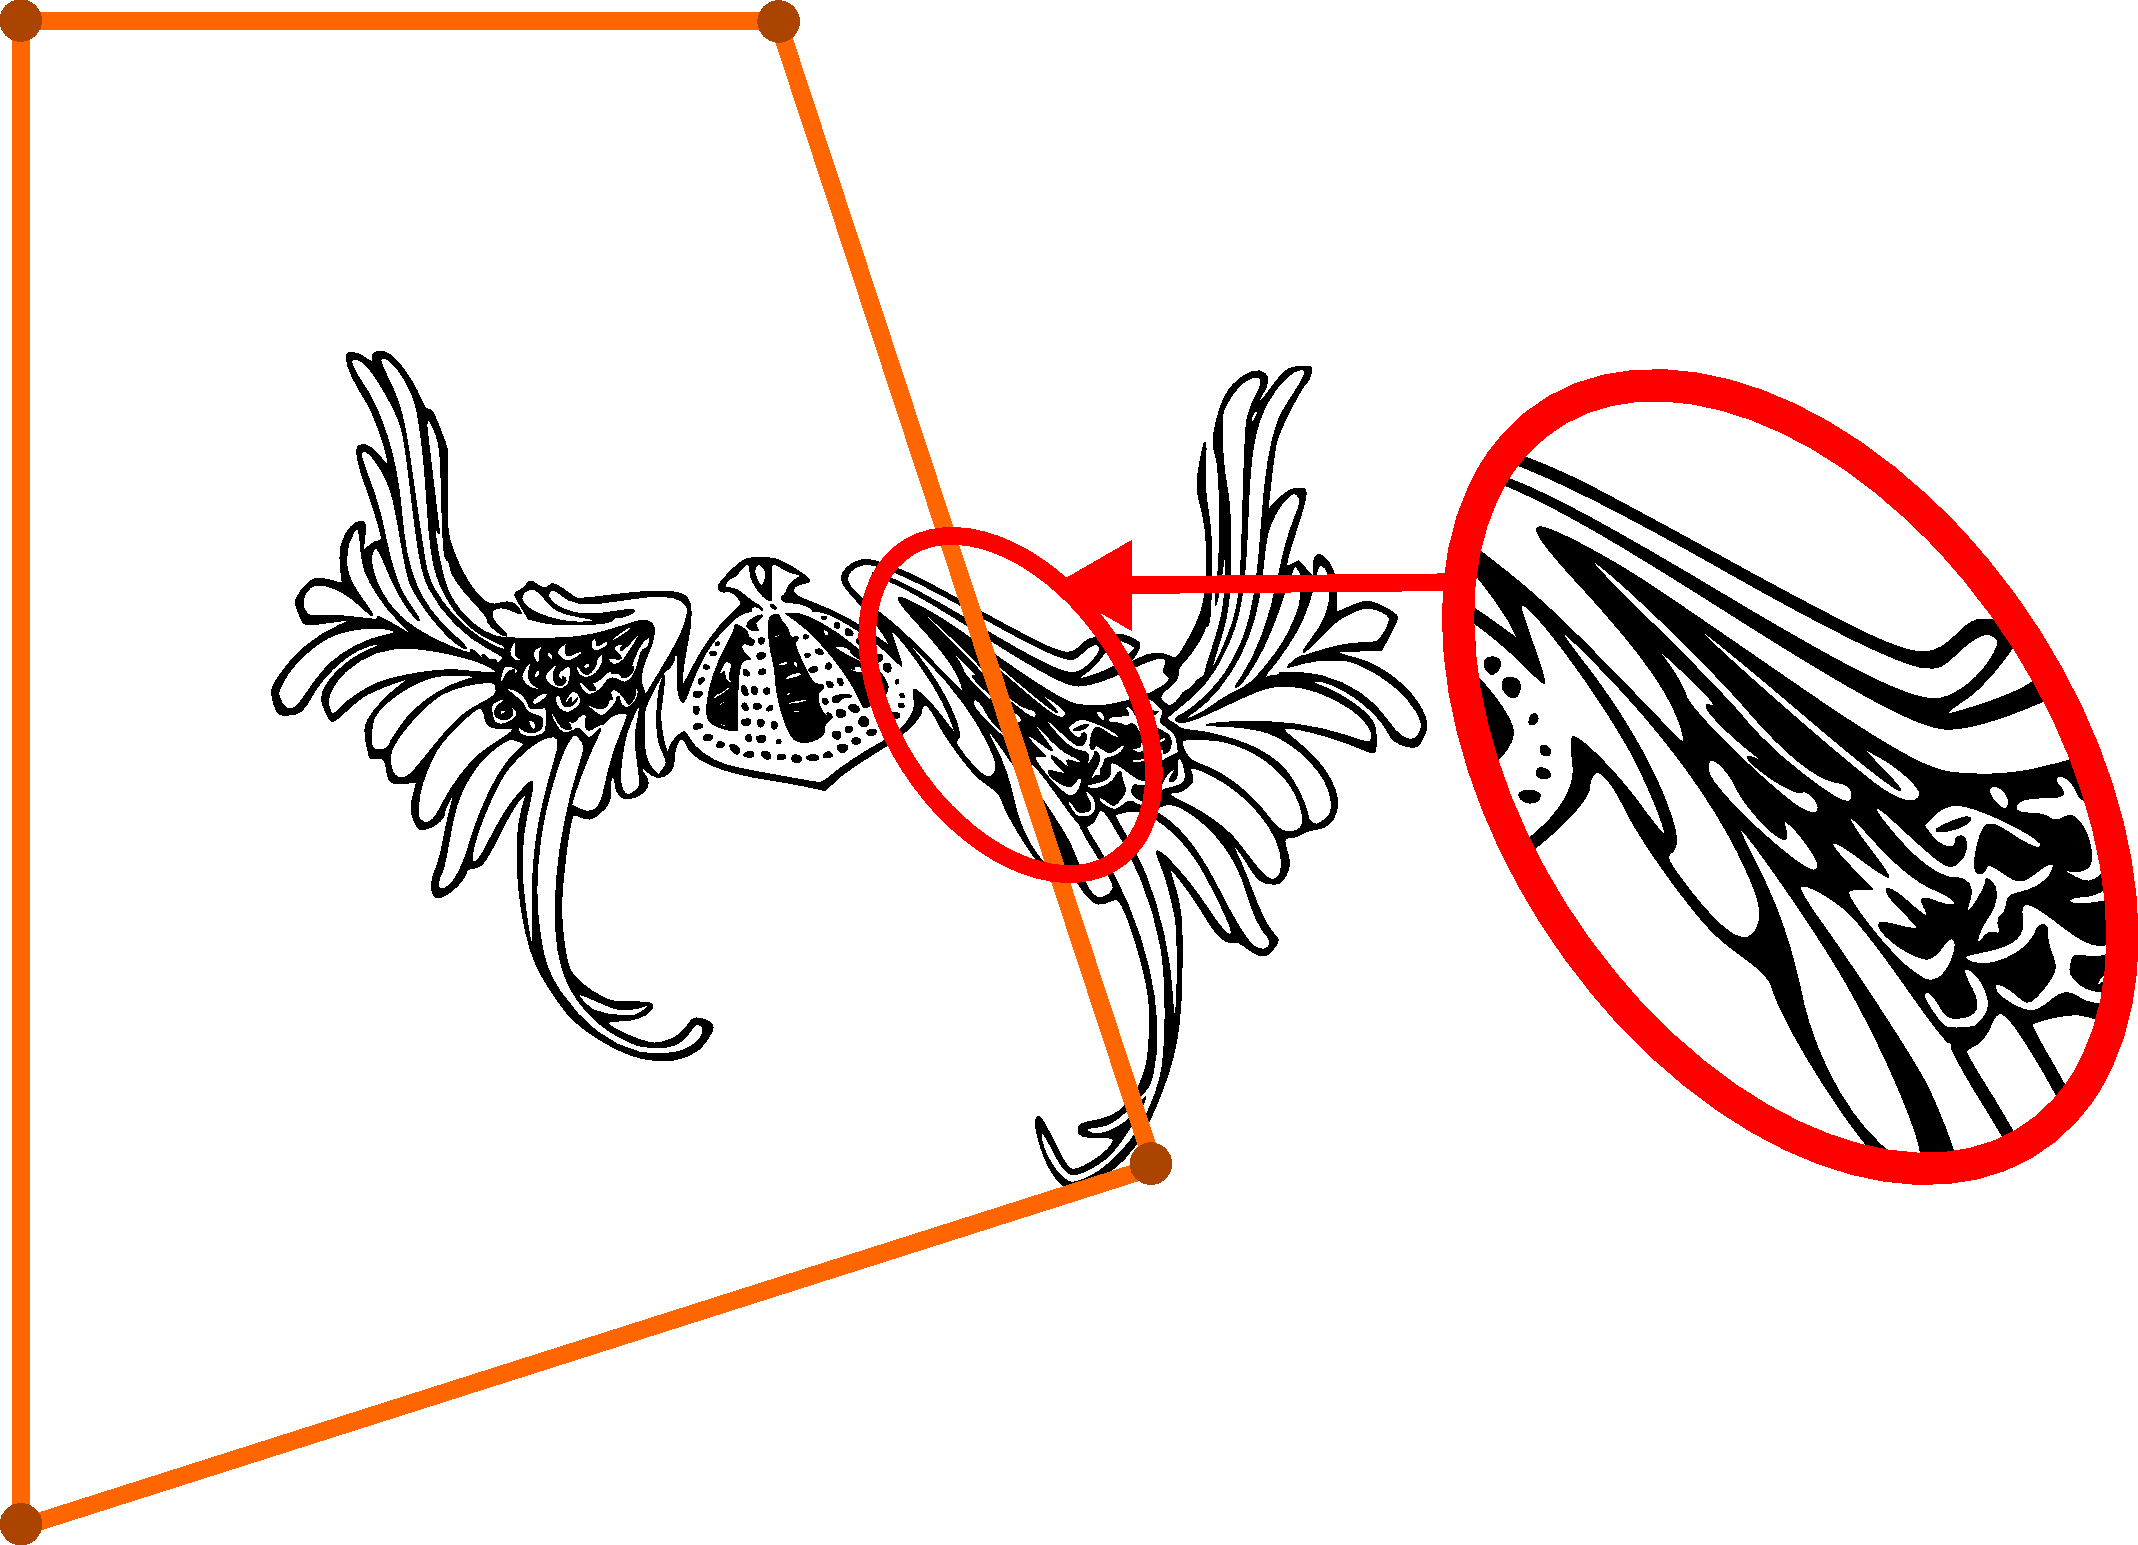
\includegraphics[scale=0.15]{Deformation-Viking-Simple-Avec}
    \end{column}
  \end{columns}
\end{frame}

\begin{frame}{Mélange d'outils}
  \centering
  \includegraphics[scale=0.3]<1>{Outil-Multi-Recouvrement-Sans-1}
  \includegraphics[scale=0.3]<2>{Outil-Multi-Recouvrement-Sans-2}
  \includegraphics[scale=0.3]<3>{Outil-Multi-Recouvrement-Avec}
\end{frame}

\begin{frame}{Mélange de déformations}
  \begin{itemize}
    \item Exprimer l'influence de la déformation de chaque outil
    \begin{displaymath}
      T_{mel}(p) = \sum_{i=1}^n D(i, p) T_{d}(i, p)
    \end{displaymath}
    \item Réutilisation de la fonction de distance $\gamma(p)$
    \begin{displaymath}
      D(i, p) = \frac{\gamma(i,p)}{\sum_{j=1}^n \gamma(j,p)}
    \end{displaymath}
  \end{itemize}
\end{frame}

\begin{frame}{Résultat du mélange}
  \begin{columns}[t]
    \begin{column}{0.5\textwidth}
      \centering
      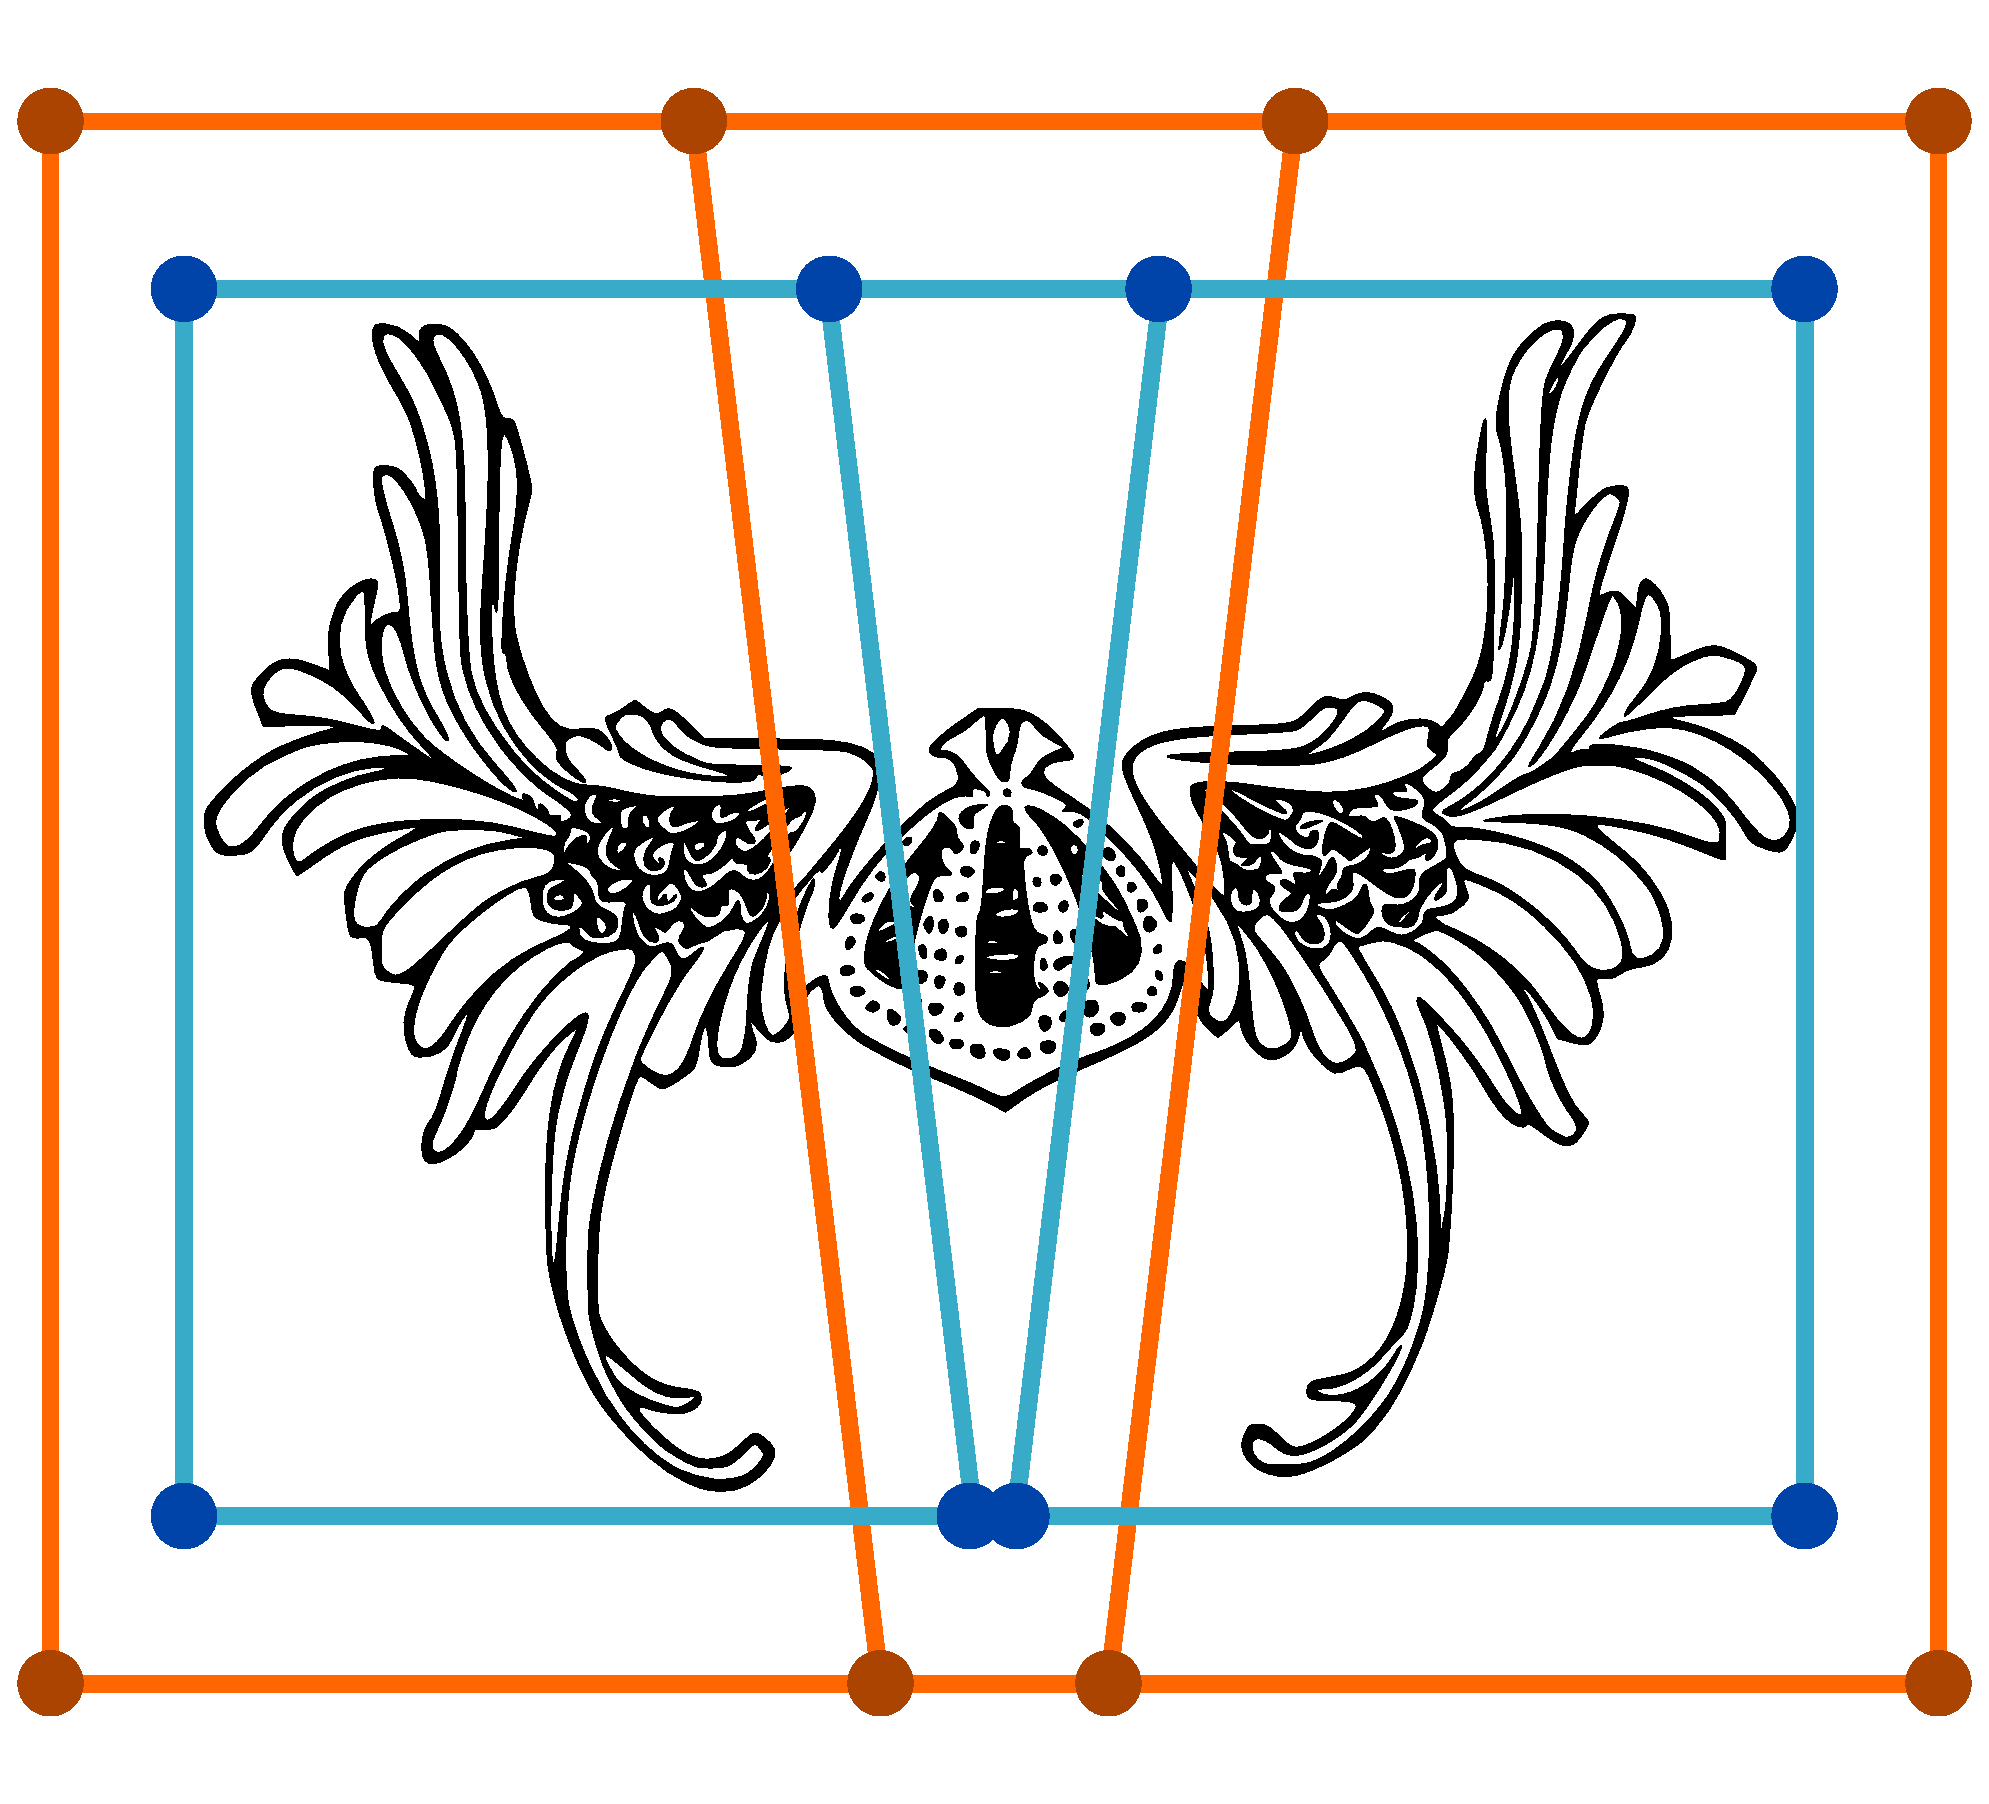
\includegraphics[scale=0.15]{Deformation-Viking-Melange-Avant}
    \end{column}
    \begin{column}{0.5\textwidth}
      \centering
      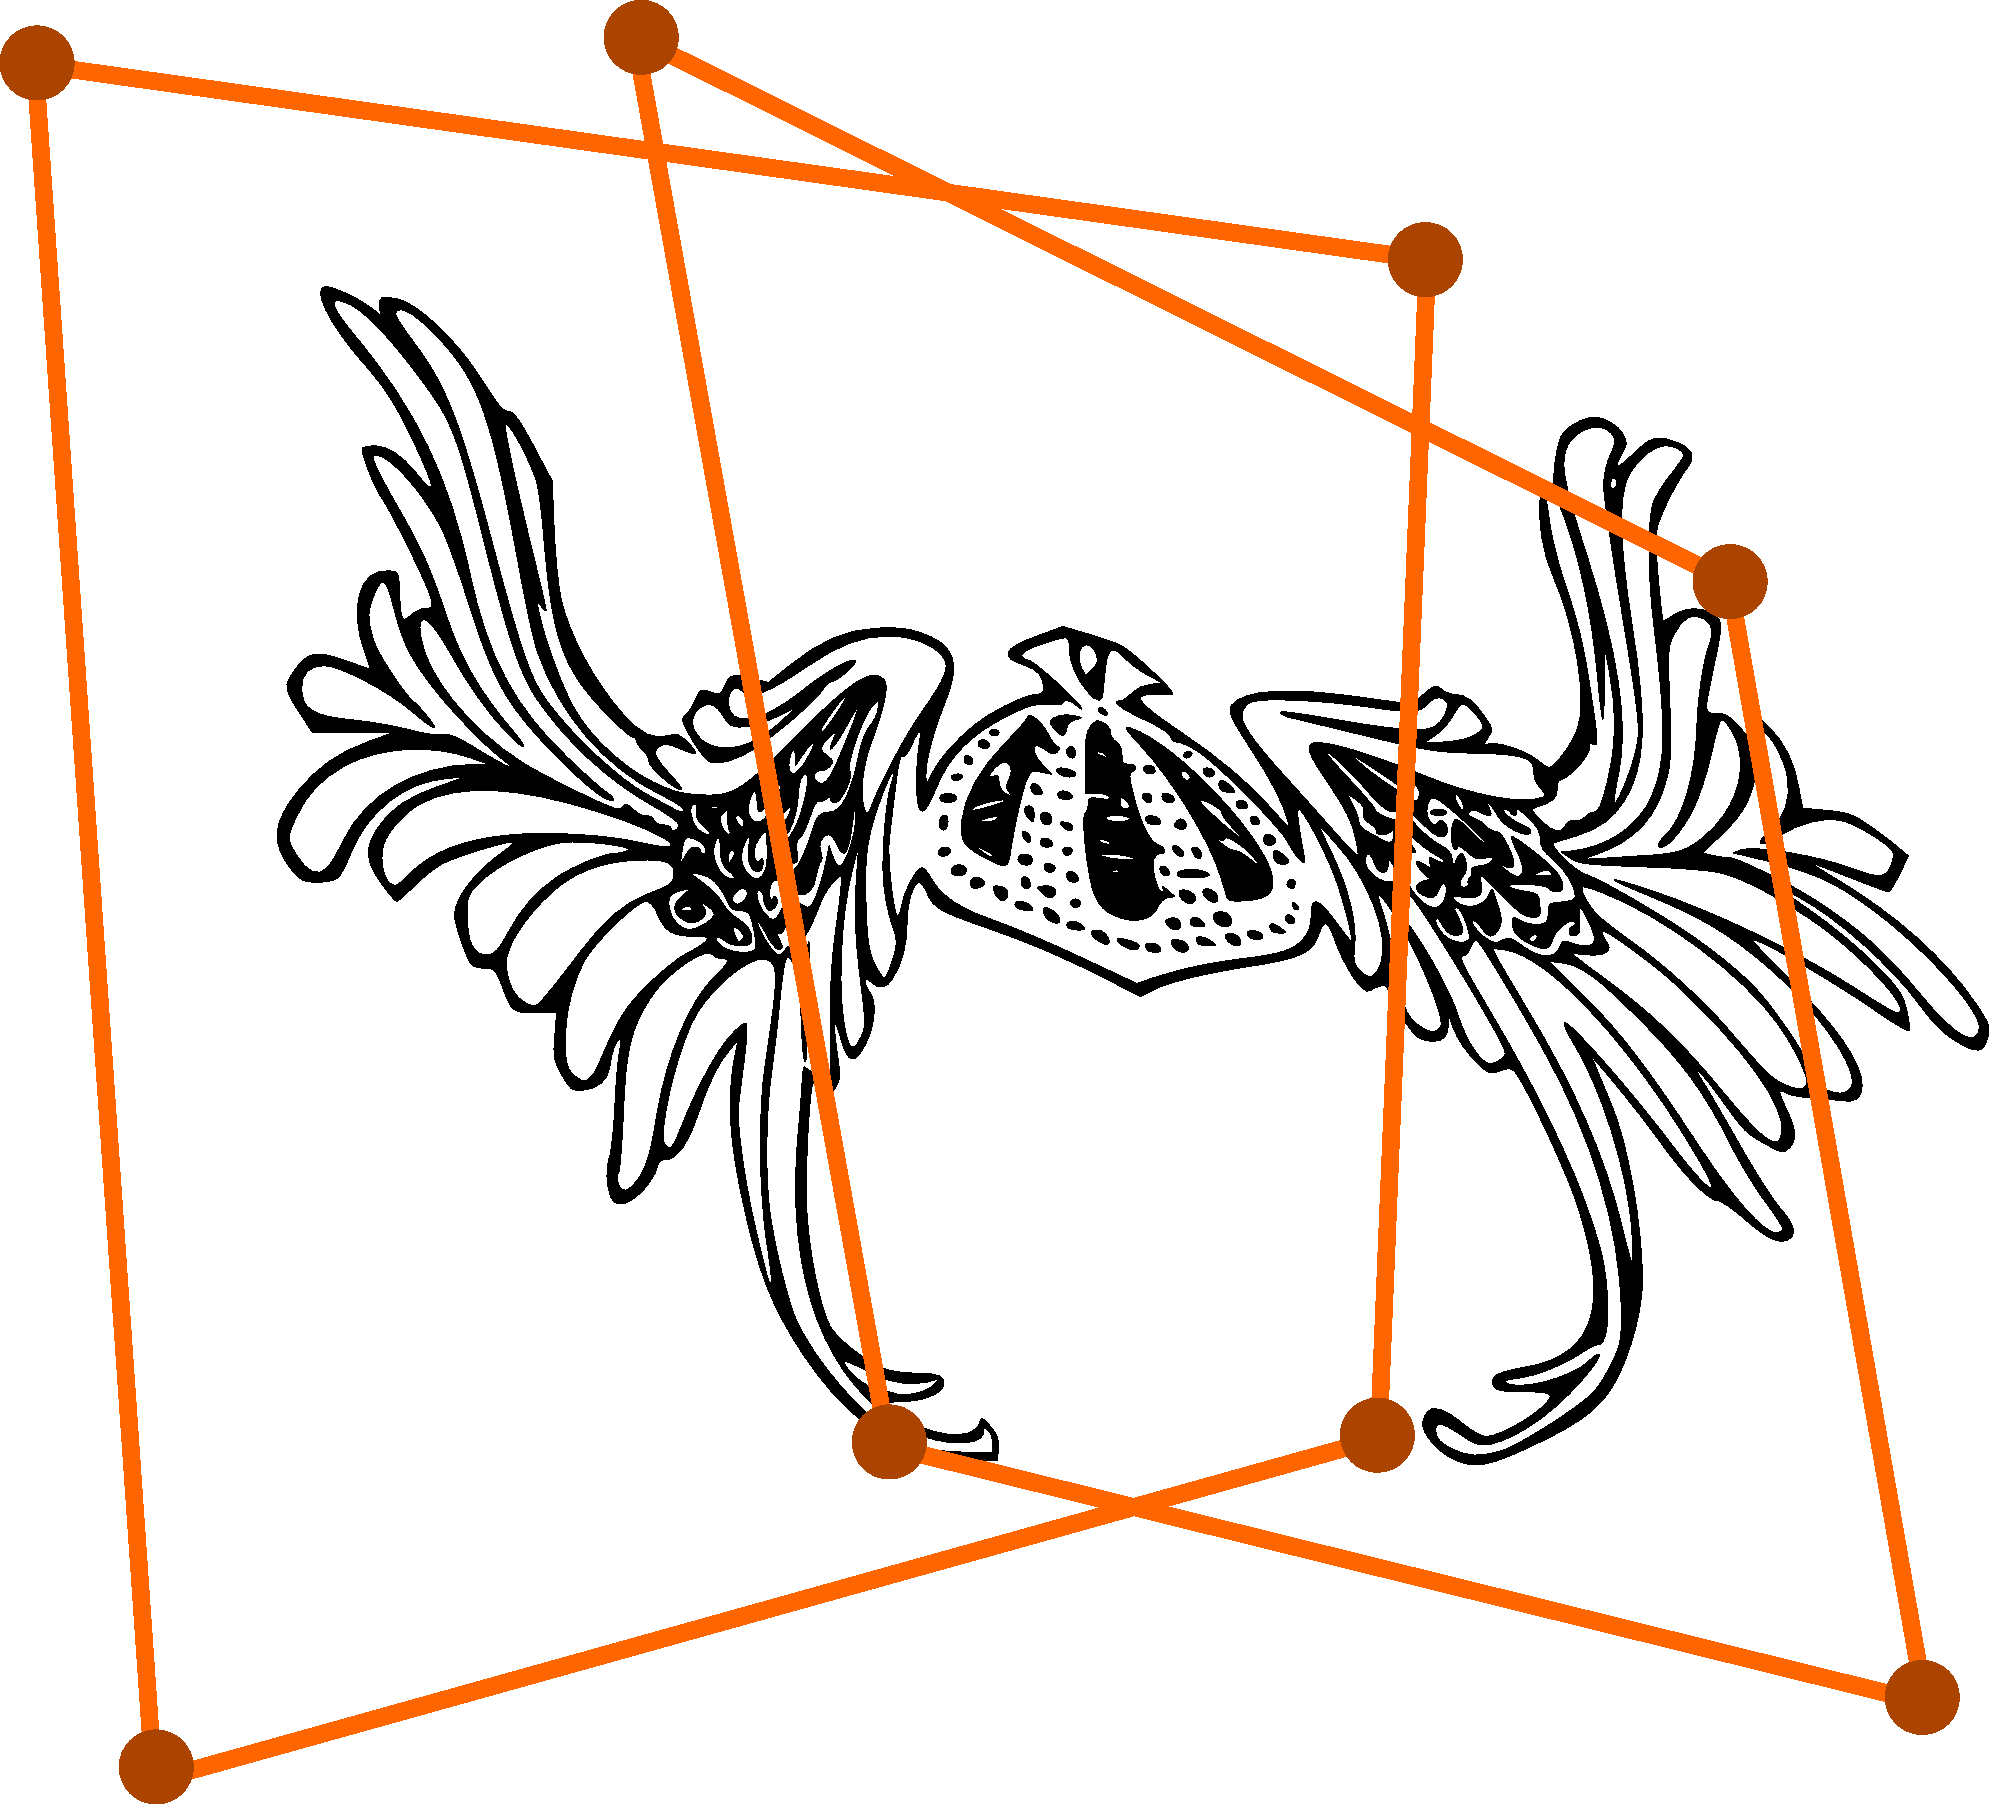
\includegraphics[scale=0.15]{Deformation-Viking-Melange-Apres}
    \end{column}
  \end{columns}
\end{frame}

\begin{frame}{Interaction utilisateur}
\centering
\movie[width=0.9\textwidth,height=0.5\paperwidth,poster,repeat,autostart,showcontrols=true]{}
{PresentationFigs/Video-DoubleCage-Grande.avi}
\end{frame}

\begin{frame}{Interaction utilisateur}
\centering
\movie[width=0.9\textwidth,height=0.5\paperwidth,poster,repeat,autostart,showcontrols=true]{}
{PresentationFigs/Video-DoubleCage-Petite.avi}
\end{frame}

\begin{frame}{Amélioration de l'interaction}
  \begin{itemize}
    \item Manipulation peu intuitive
    \item Manipuler directement la cage contrôlant l'atténuation
  \end{itemize}
  \begin{columns}[t]
    \begin{column}{0.5\textwidth}
      \centering
      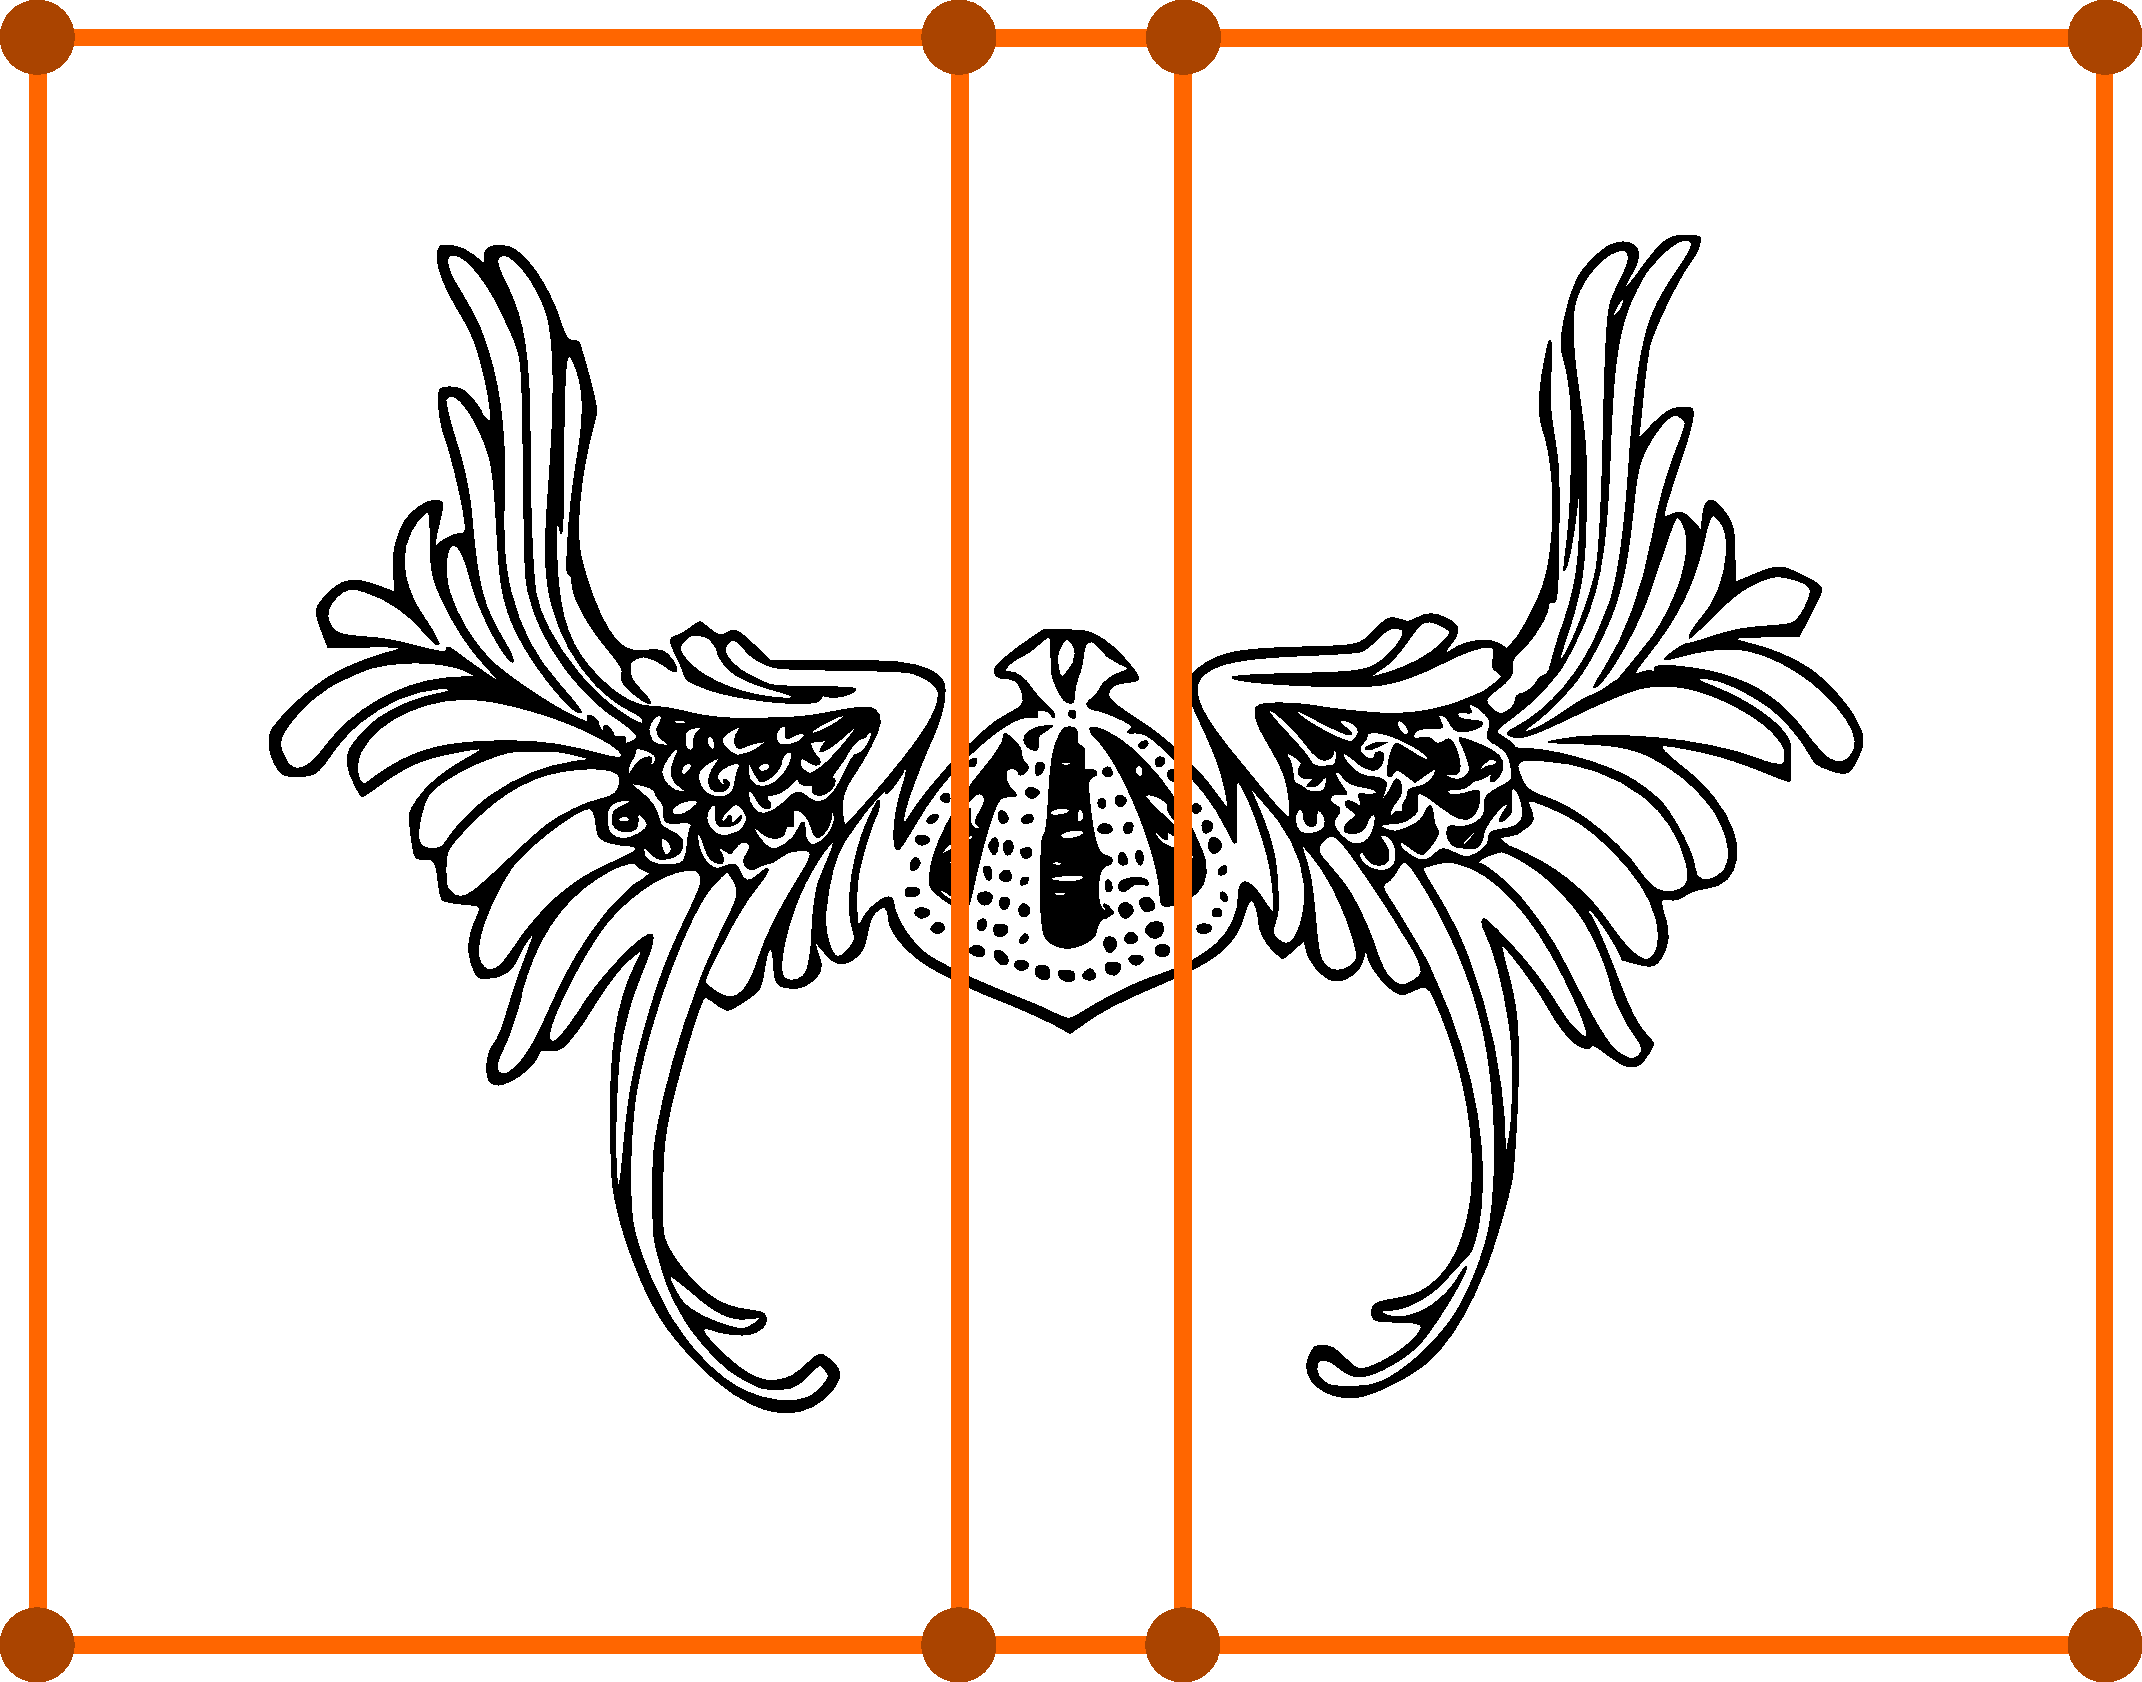
\includegraphics[scale=0.15]{Deformation-Viking-Avant}
    \end{column}
    \begin{column}{0.5\textwidth}
      \centering
      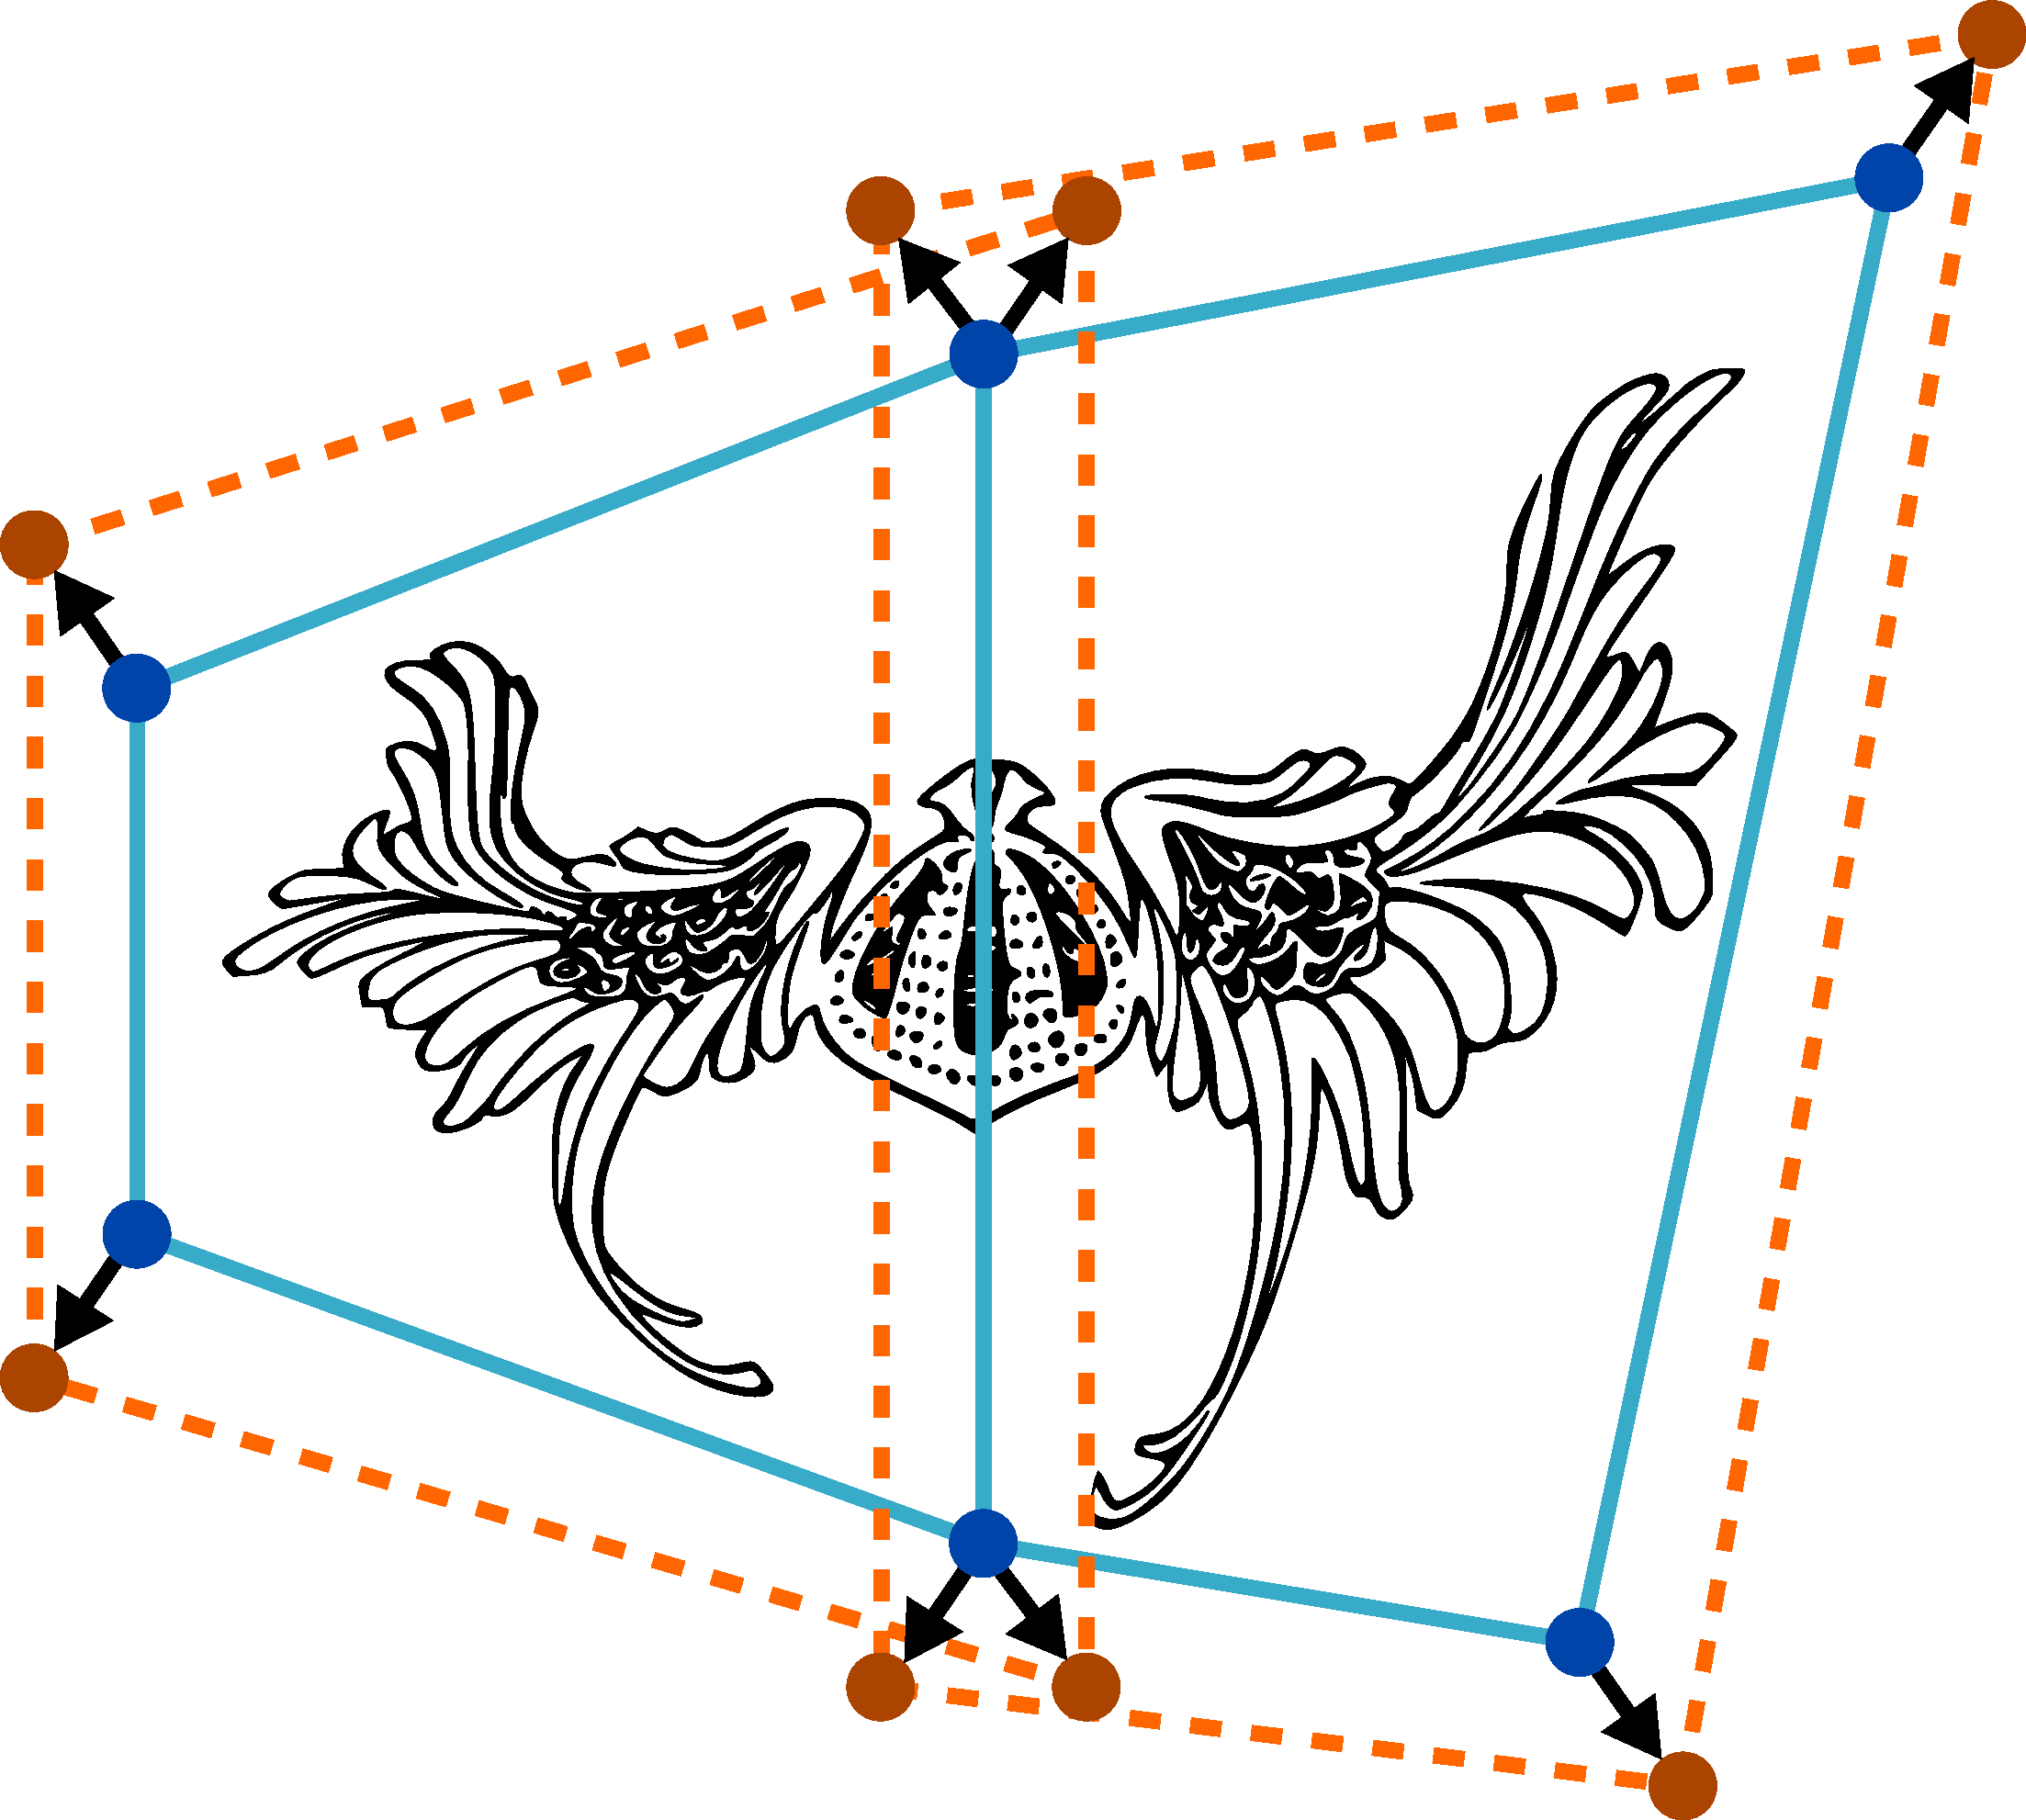
\includegraphics[scale=0.15]{Deformation-Viking-Apres-Avec}
    \end{column}
  \end{columns}
\end{frame}

\section{\scshape Conclusion}

\begin{frame}{Conclusion}
  Contributions :
  \begin{itemize}
    \item Temps d'association court
    \item Calcul de coordonnées local
    \item Atténuation rendant la déformation visuellement lisse
    \item Configuration de la zone d'atténuation
    \item Disposition quelconque des outils créés
    \item Ajout/Suppression dynamique d'outils
  \end{itemize}
  Extension directe : 
  \begin{itemize}
    \item Mélange de déformations dans $\mathbb{R}^3$
  \end{itemize}
\end{frame}

\begin{frame}{Aspect multidimensionnel}
  \begin{itemize}
    \item Point
  \end{itemize}
  \begin{columns}[t]
    \begin{column}{0.3\textwidth}
      \centering
      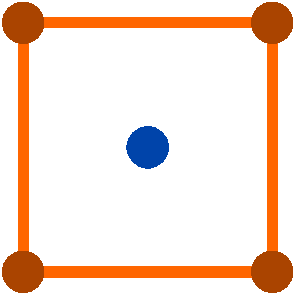
\includegraphics[scale=0.4]{OutilPoint4}
    \end{column}
    \begin{column}{0.3\textwidth}
      \centering
      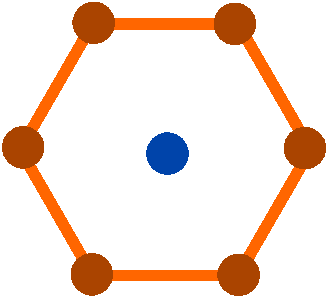
\includegraphics[scale=0.4]{OutilPoint6}
    \end{column}
    \begin{column}{0.3\textwidth}
      \centering
      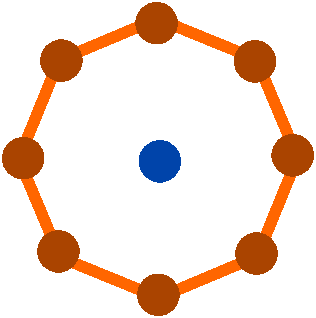
\includegraphics[scale=0.4]{OutilPoint8}
    \end{column}
  \end{columns}
  \begin{itemize}
    \item Courbe
  \end{itemize}
  \begin{columns}[t]
    \begin{column}{0.3\textwidth}
      \centering
      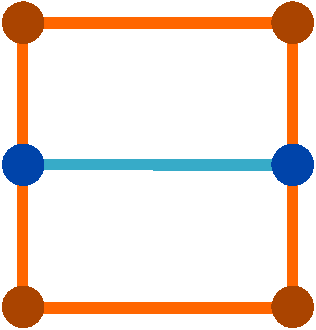
\includegraphics[scale=0.4]{OutilCourbe4}
    \end{column}
    \begin{column}{0.3\textwidth}
      \centering
      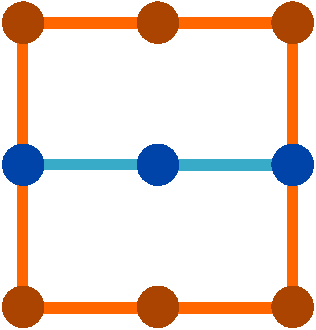
\includegraphics[scale=0.4]{OutilCourbe6}
    \end{column}
    \begin{column}{0.3\textwidth}
      \centering
      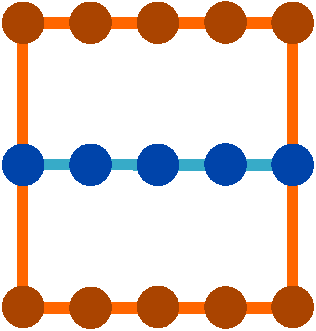
\includegraphics[scale=0.4]{OutilCourbe10}
    \end{column}
  \end{columns}
\end{frame}

\begin{frame}{}
\begin{center}
\huge Merci de votre attention.
\end{center}
\end{frame}

\appendix

\end{document}